\documentclass[conf]{new-aiaa}
%\documentclass[journal]{new-aiaa} for journal papers
\usepackage[utf8]{inputenc}

\usepackage{graphicx}
\usepackage{amsmath}
\usepackage[version=4]{mhchem}
\usepackage{siunitx}
\usepackage{longtable,tabularx}
\usepackage{footnote}
\usepackage{mhchem}
\usepackage{physics}
\usepackage{array,makecell,booktabs}
\newcolumntype{M}[1]{>{\centering\arraybackslash}m{#1}}
\usepackage[super]{nth}
\makesavenoteenv{tabular}
\setlength\LTleft{0pt} 

\graphicspath{{figures/}}


\begin{document}

\section{Classification of first stage reuse strategies}
Although only two vehicles with recoverable stages have been operated, a wide variety of first stage recovery strategies have been proposed. This section develops a systematic classification of recovery strategies.

First stage recovery strategies can be classified by four high-level choices:
\begin{enumerate}
    \item \textit{Recovery location} - The stage may return itself for recovery at the launch site, or may be recovered downrange. Launch site recovery would occur on land. Downrange recovery could occur on a ship, directly in the ocean, on land, or midair with recovered components being caught by an aircraft \cite{Ragab2015, Stappert2017}.

    \item \textit{Recovery propulsion method} - The stage may propel itself to the recovery location by firing its rocket engines or by using additional air-breathing engines. Alternatively, the stage may not use propulsion during recovery, and instead glide or fall to the recovery location.

    \item \textit{Landing method} - The stage may use rocket engines to land vertically (propulsive), land horizontally like an airplane (winged), or land under parachutes.

    \item \textit{Portion of \nth{1} stage recovered} - Some strategies recover the entire first stage, while others propose to only recover a portion containing the higher-value components (e.g. main engines \cite{Ragab2015}).
\end{enumerate}

In this paper, a "reuse strategy" will denote a combination of answers to these four choices. There are 90 possible choice combinations, of which 36 seem vaguely feasible. Of these, 11 distinct strategies have been operated or proposed (Table \ref{tab:vehicles}). Figure \ref{fig:recov_strat_diagram} illustrates the concept of operations for some of these strategies.

\begin{figure}[hbt!]
    \centering
    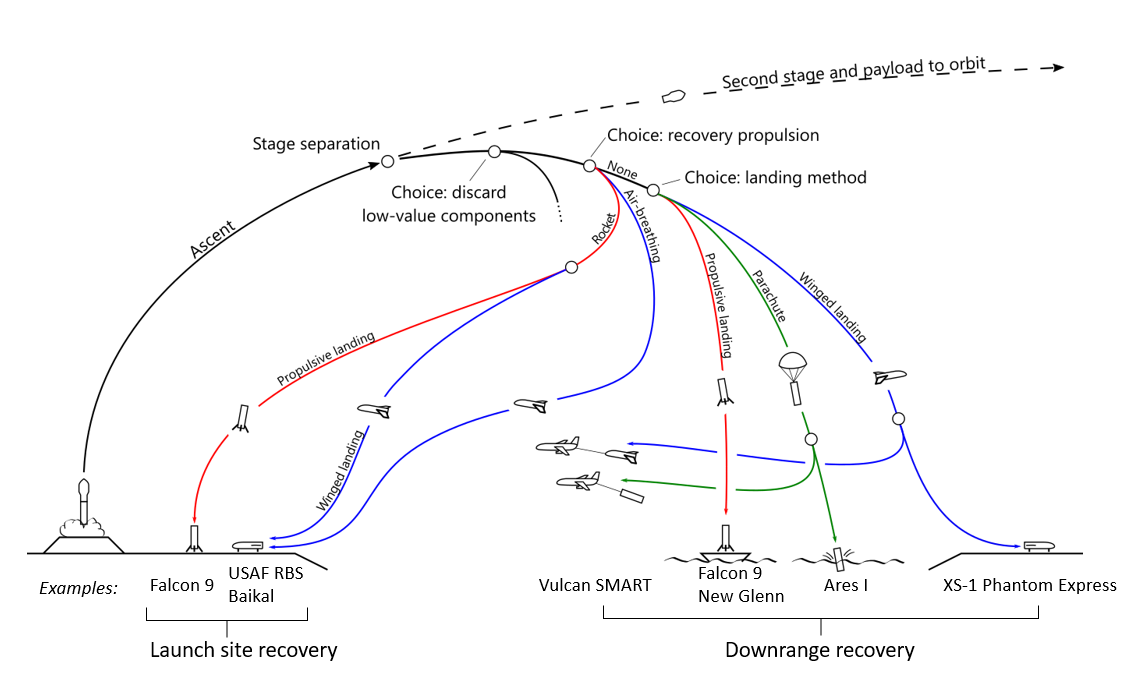
\includegraphics[width=1\textwidth]{figures/recovery_options_annotated}
    \caption{\label{fig:recov_strat_diagram} Many different strategies can be employed to recover and reuse the \nth{1} stage of a launch vehicle.}
\end{figure}

\begin{table}[hbt!]
    \caption{\label{tab:vehicles} Examples of first stage reuse strategies.}
    \centering
    \begin{tabular}{p{3.5cm} l p{2cm} p{2cm} p{2cm} p{2cm}}
        \hline
        Vehicle & Status & Recovery location & Recovery propulsion method &  Landing method & Portion of \nth{1} stage recovered \\
        \hline
        \hline
        Falcon 9 \cite{Falcon9} & Operational & Launch site or downrange & Rocket & Propulsive & Full \\
        \hline
        Space Shuttle* & Retired & Downrange & None & Parachute &  Full \\
        \hline
        New Glenn \cite{NewGlenn} & Proposed & Downrange & Rocket & Propulsive & Full \\
        XS-1 Phantom Express \cite{DARPA_XS1, Sloss18} & Proposed & Launch site or downrange & None & Winged & Full \\
        SMART (Vulcan) \cite{Ragab2015} & Proposed & Downrange (midair) & None & Parachute & Partial \\
        \hline
        Adeline (Ariane 6) & Canceled \cite{vila_dupas_2018} & Launch site & Air-breathing & Winged & Partial \\
        Ares I \cite{Ares2009} & Canceled & Downrange & None & Parachute &  Full\\
        Reusable Booster System (RBS) \cite{NAP13534} & Canceled & Launch site & Rocket & Winged & Full\\
        Kistler K-1 \cite{Isakowitz2004} & Canceled & Launch site & Rocket & parachute & Full\\ 
        NASA Liquid Fly-Back Booster (LFBB)* \cite{Healy1998} & Canceled & Launch site & Air-breathing & Winged & Full\\
        DRL Liquid Fly-Back Booster (LFBB)* \cite{Sippel2003} & Canceled & Launch site & Air-breathing & Winged & Full\\
        Baikal \cite{Isakowitz2004} & Canceled? & Launch site & Air-breathing & Winged & Full\\
        \hline
    \end{tabular}
    \\ * denotes boosters used in parallel staging.
\end{table}

The following sections will estimate the performance and cost per flight of several of the above reuse strategies.

\bibliography{first_stage_recovery}

\end{document}
